% Provenance (never printed): old terminale S material on mountain ranges and
% continental collision (folds, reverse faults and nappes as signs of
% shortening and thickening; ophiolites and sutures as the trace of a closed
% ocean; the Himalaya and the Alps as examples). Owner (Sync 0): collision,
% fold/anticline/syncline/fold axis, reverse fault/thrust, nappe, ophiolite,
% suture, shortening. Fault is Book 1's (g7), normal fault g11.05's, the root
% and Airy isostasy g11.03's and g12.01's: recalled, never redefined. India's
% past latitudes: figdata/grade-12/india_drift.py (GPlates Web Service, two
% published plate models); shortening: figdata/grade-12/fold_shortening.py;
% the belt map: figdata/grade-12/alpine_belt.py.
\chapter{पर्वतों का निर्माण}\label{ch:g12:mountain-building}

समुद्र-तल से \qty{8848.86}{m} ऊपर, माउंट एवरेस्ट की चोटी पर पहुँचने वाले पर्वतारोही
चूना पत्थर पर खड़े होते हैं। चोटी से नमूने नीचे लाने वाले भूवैज्ञानिकों को
उनमें ट्राइलोबाइटों, ऑस्ट्रैकोडों और
क्रिनॉइडों के टूटे टुकड़े मिले: समुद्री जीव जो 440 मिलियन वर्ष से भी पहले,
ऑर्डोविशियन में, रहते थे। संसार की सबसे ऊँची चट्टान किसी समुद्र की तली पर
जमी थी। यह अध्याय समझाता है कि समुद्री तली संसार की छत पर कैसे पहुँचती है:
दो महाद्वीप टकराते हैं, और उनके बीच की भूपर्पटी भिंचती है, मुड़ती है,
तहों में चढ़ती है और मोटी होकर एक पर्वत-श्रेणी बन जाती है।
% ledger: sakai05:summit, tulane:roots (marine limestones at the top of Mt. Everest), ics:base.Ordovician, ics:base.Silurian (486.85-443.1 Ma); Book 1: tht:everest (8848.86 m)

\begin{omfigure}
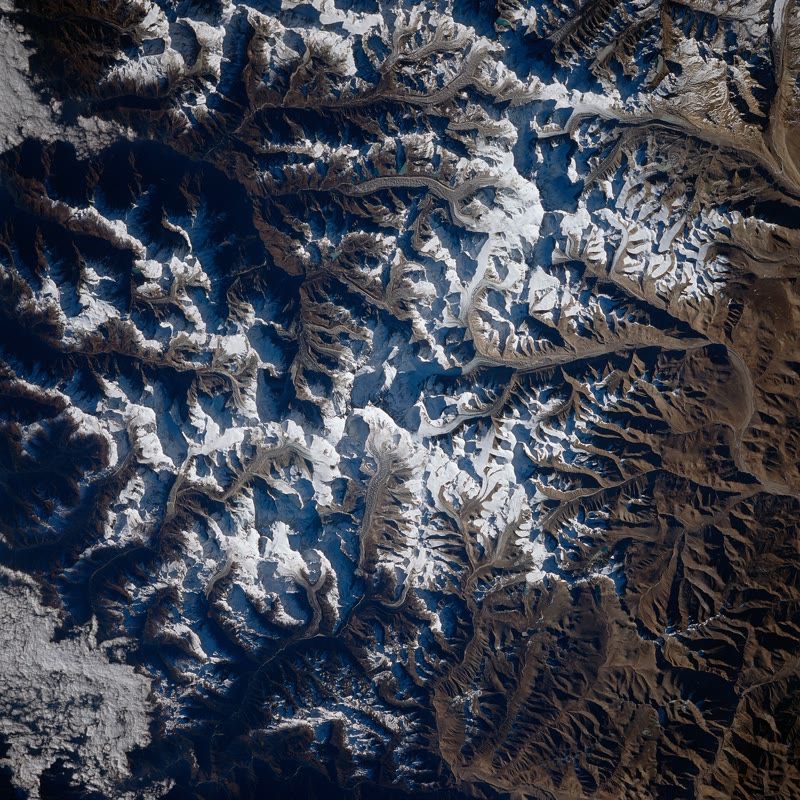
\includegraphics[width=0.5\linewidth]{images/book2/g12-nasa-everest-columbia.jpg}

{\small माउंट एवरेस्ट और उसके चारों ओर के बहुत-से हिमनद, 30 नवंबर 1996 को
अंतरिक्ष यान कोलंबिया से देखे गए। फ़ोटो नासा (सार्वजनिक डोमेन)।}
\end{omfigure}
% ledger: photo:g12-everest-columbia

\begin{recall}
किसी कटक पर बनी \omterm{def:g11:ocean-ridges:oceanic-lithosphere}{महासागरीय स्थलमंडल} की प्लेट किसी खाई पर वापस प्रावार में
डूबती है; उसकी \omterm{def:g11:subduction-zones:slab}{स्लैब} उसे नीचे खींचती है (\cref{ch:g11:subduction-zones})।
\omterm{def:g12:continental-crust:continental-crust}{महाद्वीपीय भूपर्पटी} मोटी और हल्की है, औसतन लगभग \qty{2830}{kg/m^3},
जबकि उसके नीचे के प्रावार का \qty{3380}{kg/m^3}, इसलिए वह ऊँची तैरती है, और
मोटी भूपर्पटी पतली से ऊँची खड़ी होती है, एक \omterm{def:g12:continental-crust:root}{मूल} के ऊपर
(\cref{ch:g12:continental-crust,ch:g11:lithosphere-asthenosphere})। भ्रंश
एक टूटन है जिसके अनुदिश दोनों खंड खिसके हैं; \omterm{def:g11:ocean-ridges:normal-fault}{सामान्य भ्रंश} पर
भ्रंश-तल के ऊपर का खंड नीचे खिसका है, जैसा वहाँ होता है जहाँ धीमे कटक पर
भूपर्पटी खिंचती है (\cref{ch:g11:ocean-ridges})।
\end{recall}
% ledger: cm95:crust, data:prem, tulane:no-subduct, usgs:normal-fault

\section{क्षेपण से टक्कर तक}

जो महासागर किसी खाई पर उससे तेज़ी से खपता है जितनी तेज़ी से वह अपने कटक पर बनता है, वह
सिकुड़ता है। डूबती प्लेट पर सवार कोई महाद्वीप प्लेट की चाल से खाई के
निकट आता है, और अंत में वहाँ पहुँच जाता है। उसके आगे का \omterm{def:g11:ocean-ridges:oceanic-lithosphere}{महासागरीय
स्थलमंडल} नीचे जा चुका है; महाद्वीप उसका अनुसरण नहीं कर सकता,
क्योंकि उसकी भूपर्पटी अधिक घने प्रावार में डूबने के लिए बहुत हल्की है। \omterm{def:g11:subduction-zones:subduction}{क्षेपण}
रुक जाता है। दोनों महाद्वीप एक-दूसरे से भिंच जाते हैं, और महासागरीय तली से लटकी
\omterm{def:g11:subduction-zones:slab}{स्लैब} अंततः टूटकर प्रावार में
डूब जाती है।
% ledger: earle:collision, tulane:no-subduct

\begin{definition}[महाद्वीपीय टक्कर]\label{def:g12:mountain-building:collision}
\emph{महाद्वीपीय टक्कर}\index{महाद्वीपीय टक्कर} किसी अभिसारी प्लेट-सीमा पर
दो महाद्वीपों का मिलना है, जब उनके बीच का \omterm{def:g11:ocean-ridges:oceanic-lithosphere}{महासागरीय स्थलमंडल}
क्षेपित हो चुका हो। कोई भी महाद्वीप नहीं डूबता: उनके बीच की भूपर्पटी
विकृत और मोटी होकर एक पर्वत-पट्टी बन जाती है।
\end{definition}
% ledger: earle:collision, tulane:no-subduct, usgs:himalaya-collision

\begin{omfigure}
\begin{tikzpicture}[x=0.95cm, y=0.95cm, font=\scriptsize]
  % ---- stage 1: the ocean closes ----
  \begin{scope}[yshift=0cm]
    \fill[omSea] (3.4,0) -- (8.6,0) -- (8.0,-0.5) -- (4.3,-0.5) -- (3.5,0.0) -- cycle;
    \fill[omLithGranite] (0,0.15) -- (3.5,0.15) -- (4.3,-0.5) -- (4.3,-0.75) -- (3.5,-1.0) -- (0,-1.0) -- cycle;
    \fill[omLithBasalt] (4.3,-0.5) -- (8.0,-0.5) .. controls (9.0,-0.75) and (9.6,-1.2) .. (10.4,-2.0)
      -- (10.15,-2.15) .. controls (9.4,-1.4) and (8.9,-1.0) .. (8.0,-0.75) -- (4.3,-0.75) -- cycle;
    \fill[omLithGranite] (8.0,-0.5) -- (8.6,0.2) -- (12,0.2) -- (12,-1.05) -- (9.5,-1.05)
      .. controls (9.0,-0.75) .. (8.0,-0.5) -- cycle;
    \fill[omThm!70] (10.0,0.2) -- (10.3,0.55) -- (10.6,0.2) -- cycle;
    \draw[black!60, line width=0.3pt] (0,0.15) -- (3.5,0.15) -- (4.3,-0.5) -- (8.0,-0.5) -- (8.6,0.2) -- (12,0.2);
    \draw[-{Stealth[length=2mm]}, line width=0.8pt] (1.2,0.45) -- (2.6,0.45);
    \node[anchor=east] at (0,-0.4) {1};
    \node at (1.8,-0.5) {महाद्वीप};
    \node at (6.1,-0.25) {महासागर};
    \node[anchor=north] at (6.1,-0.8) {महासागरीय स्थलमंडल};
    \node[anchor=south] at (8.0,0.0) {खाई};
    \node[anchor=south] at (10.3,0.55) {ज्वालामुखीय चाप};
    \node at (11.1,-0.5) {महाद्वीप};
  \end{scope}
  % ---- stage 2: the continents meet ----
  \begin{scope}[yshift=-3.0cm]
    \fill[omSea] (6.9,0) -- (8.4,0) -- (8.0,-0.4) -- (7.4,-0.35) -- cycle;
    \fill[omLithGranite] (0,0.15) -- (6.8,0.15) -- (7.6,-0.4) -- (8.0,-0.5)
      .. controls (9.0,-0.75) .. (9.5,-1.05) -- (9.2,-1.4) -- (6.5,-1.0) -- (0,-1.0) -- cycle;
    \fill[omLithBasalt] (9.5,-1.05) .. controls (10.0,-1.4) .. (10.6,-2.0) -- (10.35,-2.15)
      .. controls (9.8,-1.6) .. (9.2,-1.4) -- cycle;
    \fill[omLithGranite] (8.0,-0.5) -- (8.6,0.2) -- (12,0.2) -- (12,-1.05) -- (9.5,-1.05)
      .. controls (9.0,-0.75) .. (8.0,-0.5) -- cycle;
    \fill[omLithPeridotite] (7.0,0.15) -- (7.9,0.15) -- (8.3,0.05) -- (7.95,-0.12) -- (7.3,0.0) -- cycle;
    \fill[omThm!70] (10.0,0.2) -- (10.3,0.55) -- (10.6,0.2) -- cycle;
    \draw[-{Stealth[length=2mm]}, line width=0.8pt] (3.2,0.45) -- (4.6,0.45);
    \node[anchor=east] at (0,-0.4) {2};
    \node at (3.4,-0.45) {महाद्वीप};
    \draw[black!60] (7.6,0.12) -- (7.0,0.75) node[anchor=south east, inner sep=1pt] {महासागरीय तली की फाँक};
    \node at (11.1,-0.5) {महाद्वीप};
    \node[anchor=west] at (10.7,-1.9) {स्लैब};
  \end{scope}
  % ---- stage 3: a mountain belt ----
  \begin{scope}[yshift=-6.4cm]
    \fill[omLithGranite] (0,0.15) -- (4.5,0.15) .. controls (6.0,0.4) and (6.6,1.25) .. (7.6,1.3)
      .. controls (8.7,1.3) and (9.6,0.5) .. (10.6,0.2) -- (12,0.2) -- (12,-1.05) -- (10.6,-1.1)
      .. controls (9.5,-2.2) and (8.6,-2.6) .. (7.7,-2.6) .. controls (6.6,-2.6) and (5.6,-1.6) .. (4.5,-1.0)
      -- (0,-1.0) -- cycle;
    \draw[black!60, line width=0.3pt] (0,0.15) -- (4.5,0.15) .. controls (6.0,0.4) and (6.6,1.25) .. (7.6,1.3)
      .. controls (8.7,1.3) and (9.6,0.5) .. (10.6,0.2) -- (12,0.2);
    \draw[black!60, dashed, line width=0.4pt] (0,-1.0) -- (4.5,-1.0) .. controls (5.6,-1.6) and (6.6,-2.6) .. (7.7,-2.6)
      .. controls (8.6,-2.6) and (9.5,-2.2) .. (10.6,-1.1) -- (12,-1.05);
    \draw[omThm, line width=1.0pt] (7.0,1.25) -- (8.3,-2.55);
    \foreach \t in {0.15,0.4,0.65}
      \fill[omLithPeridotite] ($(7.0,1.25)!\t!(8.3,-2.55)$) ++(-0.12,0.05) -- ++(0.3,0) -- ++(-0.05,-0.22) -- ++(-0.3,0) -- cycle;
    \fill[omLithBasalt] (10.9,-1.9) -- (11.5,-2.35) -- (11.35,-2.5) -- (10.75,-2.05) -- cycle;
    \node[anchor=east] at (0,-0.4) {3};
    \node at (2.4,-0.45) {महाद्वीप};
    \node at (11.3,-0.5) {महाद्वीप};
    \draw[black!60] (7.2,0.6) -- (5.9,1.5) node[anchor=east, inner sep=1pt] {ओफ़ियोलाइटों सहित सीवन};
    \node at (7.7,-1.9) {मूल};
    \node[anchor=north] at (11.2,-2.5) {टूटकर अलग हुई स्लैब};
    \node[anchor=south] at (7.6,1.35) {पर्वत-पट्टी};
  \end{scope}
\end{tikzpicture}

{\small \omterm{def:g11:subduction-zones:subduction}{क्षेपण} से टक्कर तक (पैमाने पर नहीं)। 1: कोई महासागर बंद होता है, जब
उसकी तली किसी खाई पर डूबती है। 2: महाद्वीप खाई तक पहुँचता है और
डूब नहीं सकता; महासागरीय तली की फाँकें उसके किनारे पर धकेल दी जाती हैं। 3: दोनों
महाद्वीपों के बीच की भूपर्पटी छोटी और मोटी होकर एक \omterm{def:g12:continental-crust:root}{मूल} के ऊपर खड़ी
पर्वत-पट्टी बन जाती है; वह रेखा जहाँ दोनों महाद्वीप जुड़े हैं, जिसे
महासागरीय तली की फाँकें चिह्नित करती हैं, \omterm{def:g12:mountain-building:suture}{सीवन} है; \omterm{def:g11:subduction-zones:slab}{स्लैब} टूटकर डूब जाती है।}
\end{omfigure}
% ledger: earle:collision, tulane:ocean-basins, usgs:suture, tulane:roots

\subsection{लुप्त महासागर का चिह्न}

जब महासागर बंद हो जाता है, तो दोनों महाद्वीप एक रेखा के अनुदिश जुड़ जाते हैं।

\begin{definition}[सीवन]\label{def:g12:mountain-building:suture}
\emph{सीवन}\index{सीवन} वह रेखा, या संकरा क्षेत्र, है जिसके अनुदिश दो
महाद्वीप किसी टक्कर द्वारा, उनके बीच \omterm{def:g11:subduction-zones:subduction}{क्षेपण} रुक जाने के बाद, जुड़े हैं:
किसी पूर्व प्लेट-सीमा का चिह्न। यह दिखाती है कि उनके बीच का महासागर
कहाँ हुआ करता था।
\end{definition}
% ledger: usgs:suture, liu20:itsz

\omterm{def:g12:mountain-building:suture}{सीवन} को क्या चिह्नित करता है? उनमें से बहुतों के अनुदिश चट्टानों के ऐसे पिंड पड़े हैं जो
किसी महाद्वीप पर कहीं के नहीं हैं: ऊपर से नीचे, समुद्री अवसाद, तकिया
बेसाल्ट, अगल-बगल खड़े ऊर्ध्वाधर \omterm{def:g11:igneous-rocks:intrusion}{डाइकों} का एक पुंज, \omterm{def:g11:ocean-ridges:gabbro}{गैब्रो}, और
आधार पर प्रावार का \omterm{def:g11:ocean-ridges:peridotite}{पेरिडोटाइट}: महासागरीय तली की परतें
(\cref{ch:g11:ocean-ridges}), उनके नीचे प्रावार के शीर्ष के साथ।
% ledger: tulane:ocean-basins

\begin{definition}[ओफ़ियोलाइट]\label{def:g12:mountain-building:ophiolite}
\emph{ओफ़ियोलाइट}\index{ओफ़ियोलाइट} \omterm{def:g11:ocean-ridges:oceanic-lithosphere}{महासागरीय स्थलमंडल} का एक टुकड़ा है ---
अवसाद, तकिया बेसाल्ट, चादरी \omterm{def:g11:igneous-rocks:intrusion}{डाइक}, \omterm{def:g11:ocean-ridges:gabbro}{गैब्रो} और प्रावार का \omterm{def:g11:ocean-ridges:peridotite}{पेरिडोटाइट} ---
जो \omterm{def:g12:continental-crust:continental-crust}{महाद्वीपीय भूपर्पटी} पर धकेल दिया गया हो।
\end{definition}
% ledger: tulane:ocean-basins

\omterm{def:g12:mountain-building:ophiolite}{ओफ़ियोलाइट} फँसी हुई महासागरीय तली है: लुप्त महासागर की एक फाँक, जो
बाक़ी के साथ डूबने के बजाय किसी महाद्वीप पर धकेल दी गई। टक्कर से उठे
पर्वतों में सामान्यतः कुछ \omterm{def:g11:ocean-ridges:oceanic-lithosphere}{महासागरीय भूपर्पटी} और ऊपरी प्रावार होता है, क्योंकि वहीं
कोई महासागर बंद हुआ था। दक्षिणी तिब्बत में, सिंधु--त्सांगपो \omterm{def:g12:mountain-building:suture}{सीवन} के अनुदिश
फैले \omterm{def:g12:mountain-building:ophiolite}{ओफ़ियोलाइट} नव-टेथिस नामक एक महासागर के अवशेष हैं, जो
भारत और ल्हासा के क्षेत्र के बीच था; वहाँ के एक \omterm{def:g11:ocean-ridges:gabbro}{गैब्रो} की आयु
243 मिलियन वर्ष आँकी गई है।
% ledger: tulane:ocean-basins, earle:collision, liu20:itsz

\begin{omfigure}
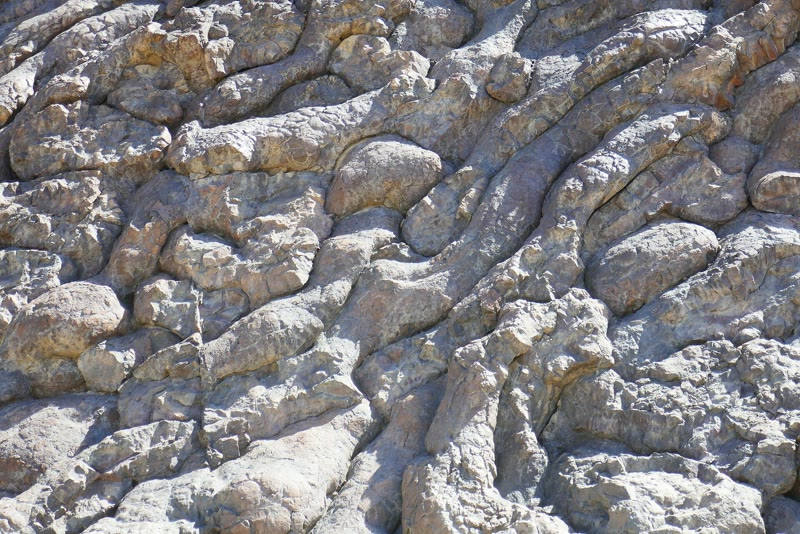
\includegraphics[width=0.6\linewidth]{images/book2/g12-duchoiselle-oman-pillows.jpg}

{\small ओमान के वादी जिज़्ज़ी में सेमाइल \omterm{def:g12:mountain-building:ophiolite}{ओफ़ियोलाइट} का तकिया लावा: वह लावा जो
पानी के नीचे गोल तकियों के रूप में ठंडा हुआ, अब स्थल पर है। फ़ोटो लियोनेल
द्यूशुआज़ेल (CC~BY-SA~3.0)।}
\end{omfigure}
% ledger: photo:g12-oman-pillows

\section{भूपर्पटी का लघुकरण}

किनारों से भींचे जाने पर चट्टान का कोई पिंड, यदि वह ठंडा और भंगुर है, तो टूट जाता है; यदि
वह प्लास्टिक ढंग से व्यवहार करने लायक गरम है, तो मुड़ जाता है। पर्वत-पट्टी
\omterm{def:g12:mountain-building:fold}{वलनों} और भ्रंशों दोनों से भरी होती है।
% ledger: earle:folds

\subsection{वलन}

\begin{definition}[वलन; अपनति; अभिनति; वलन-अक्ष]\label{def:g12:mountain-building:fold}
\emph{वलन}\index{वलन} चट्टान की परतों में एक मोड़ है। उसकी ढलवाँ भुजाएँ
\emph{भुजाएँ} कहलाती हैं; वे \emph{कब्ज़े} पर मिलती हैं, जहाँ परतें सबसे अधिक
मुड़ी होती हैं, और कब्ज़े के अनुदिश की रेखा
\emph{वलन-अक्ष}\index{वलन-अक्ष} है। \emph{अपनति}\index{अपनति} वह वलन है जिसकी परतें
ऊपर की ओर मुड़ती हैं, उसकी भुजाएँ अक्ष से दूर नत होती हैं;
\emph{अभिनति}\index{अभिनति} वह वलन है जिसकी परतें नीचे की ओर मुड़ती हैं, उसकी
भुजाएँ अक्ष की ओर नत होती हैं।
\end{definition}
% ledger: earle:folds, tulane:fold-geometry

क्रमागत परतों के कब्ज़ों से होकर जाने वाला तल अक्षीय तल है।
\omterm{def:g12:mountain-building:fold}{अपनतियाँ} और \omterm{def:g12:mountain-building:fold}{अभिनतियाँ} सामान्यतः जोड़ियों में आती हैं, एक की भुजा अगले की
भुजा होती है। \omterm{def:g12:mountain-building:fold}{वलन} हर आकार के होते हैं, सूक्ष्मदर्शीय से लेकर दसियों
किलोमीटर चौड़े तक। अपरदित होने पर \omterm{def:g12:mountain-building:fold}{अपनति} अपने क्रोड में अपनी सबसे पुरानी परतें
दिखाती है और \omterm{def:g12:mountain-building:fold}{अभिनति} अपनी सबसे नई; \omterm{def:g12:mountain-building:fold}{अपनति} आवश्यक रूप से कटक
नहीं होती, न \omterm{def:g12:mountain-building:fold}{अभिनति} घाटी, क्योंकि अपरदन \omterm{def:g12:mountain-building:fold}{वलन} की आकृति के बजाय कठोर और
नरम परतों का अनुसरण करता है।
% ledger: earle:folds, tulane:fold-geometry

\begin{omfigure}
\begin{tikzpicture}[x=1.2cm, y=1.2cm, font=\scriptsize]
  \def\W{6}\def\H{2.0}\def\dx{1.35}\def\dy{0.78}
  \tikzset{declare function={zb(\x,\c)=\c+0.8*cos(60*(\x-1.5));}}
  \colorlet{bandA}{omLithSchist!70}\colorlet{bandB}{omLithSand}\colorlet{bandC}{omLithShale}
  \colorlet{bandD}{icsJurassic!35}\colorlet{bandE}{icsTriassic!35}\colorlet{bandF}{icsCretaceous!45}
  % front face
  \begin{scope}
    \clip (0,0) rectangle (\W,\H);
    \fill[bandA] (0,0) rectangle (\W,\H);
    \foreach \c/\col in {0.0/bandB, 0.6/bandC, 1.2/bandD, 1.8/bandE, 2.4/bandF}
      \fill[\col] plot[domain=0:\W, samples=80, smooth] (\x,{zb(\x,\c)}) -- (\W,4) -- (0,4) -- cycle;
    \foreach \c in {0.0,0.6,1.2,1.8,2.4}
      \draw[black!55, line width=0.35pt] plot[domain=0:\W, samples=80, smooth] (\x,{zb(\x,\c)});
  \end{scope}
  % top face: outcrop bands (crossings of the top surface computed for these curves)
  \fill[bandE] (0,\H) -- (0.242,\H) -- ++(\dx,\dy) -- (\dx,\H+\dy) -- cycle;
  \fill[bandD] (0.242,\H) -- (2.758,\H) -- ++(\dx,\dy) -- (0.242+\dx,\H+\dy) -- cycle;
  \fill[bandE] (2.758,\H) -- (3.5,\H) -- ++(\dx,\dy) -- (2.758+\dx,\H+\dy) -- cycle;
  \fill[bandF] (3.5,\H) -- (5.5,\H) -- ++(\dx,\dy) -- (3.5+\dx,\H+\dy) -- cycle;
  \fill[bandE] (5.5,\H) -- (\W,\H) -- ++(\dx,\dy) -- (5.5+\dx,\H+\dy) -- cycle;
  \foreach \x in {0.242,2.758,3.5,5.5} \draw[black!55, line width=0.35pt] (\x,\H) -- ++(\dx,\dy);
  % right face: the layers meet it at constant heights (cylindrical folds)
  \foreach \lo/\hi/\col in {0.0/0.6/bandB, 0.6/1.2/bandC, 1.2/1.8/bandD, 1.8/2.0/bandE}
    \fill[\col] (\W,\lo) -- (\W+\dx,\lo+\dy) -- (\W+\dx,\hi+\dy) -- (\W,\hi) -- cycle;
  \foreach \y in {0.6,1.2,1.8} \draw[black!55, line width=0.35pt] (\W,\y) -- ++(\dx,\dy);
  % outline
  \draw[black, line width=0.5pt] (0,0) rectangle (\W,\H) (0,\H) -- (\dx,\H+\dy) -- (\W+\dx,\H+\dy) -- (\W,\H)
    (\W+\dx,\H+\dy) -- (\W+\dx,\dy) -- (\W,0);
  % fold axes on the top face, axial planes on the front face
  \draw[omThm, line width=1pt] (1.5,\H) -- ++(\dx,\dy);
  \draw[omDef, line width=1pt] (4.5,\H) -- ++(\dx,\dy);
  \draw[omThm, dashed, line width=0.6pt] (1.5,0) -- (1.5,\H);
  \draw[omDef, dashed, line width=0.6pt] (4.5,0) -- (4.5,\H);
  \node[anchor=south, omThm] at (1.5+\dx,\H+\dy) {अपनति: वलन-अक्ष};
  \node[anchor=south, omDef] at (4.5+\dx,\H+\dy) {अभिनति: वलन-अक्ष};
  \draw[black!70] (3.2,0.95) -- (3.9,-0.35) node[anchor=north] {भुजा};
  \draw[black!70] (1.5,1.4) circle (0.07) -- (0.4,-0.35) node[anchor=north] {कब्ज़ा};
  \draw[black!70] (1.5,0.25) -- (2.0,-0.35) node[anchor=north] {अक्षीय तल};
\end{tikzpicture}

{\small एक समतल अपरदित सतह से कटी एक \omterm{def:g12:mountain-building:fold}{अपनति} और एक \omterm{def:g12:mountain-building:fold}{अभिनति} (खंड-आरेख,
पैमाने पर नहीं)। \omterm{def:g12:mountain-building:fold}{वलन-अक्ष} कब्ज़ों के अनुदिश चलते हैं; धराशायी
रेखाएँ अक्षीय तलों के चिह्न हैं। ऊपरी सतह पर अपरदित
\omterm{def:g12:mountain-building:fold}{अपनति} अपने क्रोड में पुरानी परतें दिखाती है, \omterm{def:g12:mountain-building:fold}{अभिनति} नई।}
\end{omfigure}
% ledger: earle:folds, tulane:fold-geometry

\begin{omfigure}
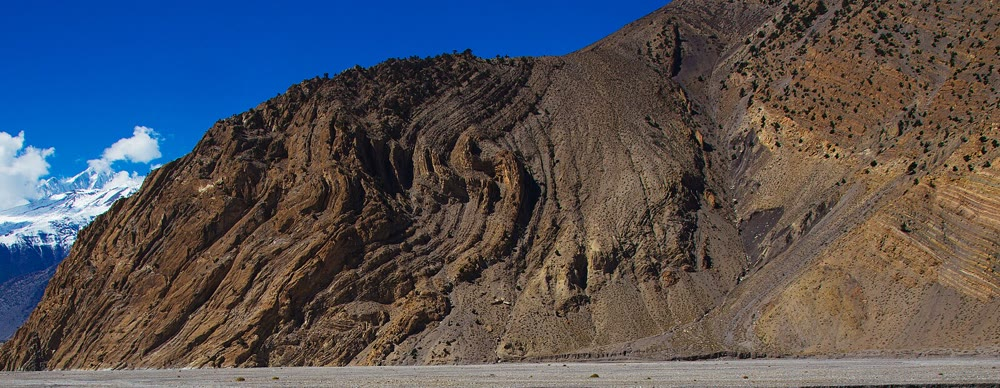
\includegraphics[width=0.95\linewidth]{images/book2/g12-hullot-kali-gandaki-folds.jpg}

{\small हिमालय की एक खड़ी चट्टान में मुड़ी हुई चट्टानी परतें, नेपाल में काली गंडकी
महाखड्ड में जोमसोम से लगभग \qty{3}{km} उत्तर-पूर्व।
फ़ोटो ज़ाँ-मारी उलो (CC~BY~2.0)।}
\end{omfigure}
% ledger: photo:g12-kali-gandaki

वार्डन पहाड़ियों का आवरण भी इसी तरह मुड़ा है, कहीं अधिक मंद रूप से।
उसके बलुआ पत्थर, चूना पत्थर, शेल और खड़िया समतल जमे थे, फिर मुड़कर
एक \omterm{def:g12:mountain-building:fold}{अपनति} और एक \omterm{def:g12:mountain-building:fold}{अभिनति} बन गए जिनकी भुजाएँ \ang{12} नत हैं; बाद का एक \omterm{def:g11:ocean-ridges:normal-fault}{सामान्य
भ्रंश} उन्हें काटता है।
% ledger: region:name; model in figdata/shared/region.py (LIMB_DIP 12, AXIS_ANTI 3.5 km, AXIS_SYN 7.5 km)

\begin{omfigure}
\begin{tikzpicture}
\begin{axis}[omsection, x=1.25cm, y=0.003125cm, xmin=0, xmax=9.49, ymin=-700, ymax=650,
  xlabel={A से दूरी (\unit{km})}, ylabel={ऊँचाई (\unit{m})},
  ytick={-600,-300,0,300,600}, tick label style={font=\scriptsize}]
\addplot[fill=black!8, draw=black!50, line width=0.3pt, even odd rule] table {figdata/out/shared-region-section-unit-schist.dat};
\addplot[fill=icsTriassic!20, draw=black!50, line width=0.3pt, even odd rule] table {figdata/out/shared-region-section-unit-sandstone.dat};
\addplot[fill=icsJurassic!25, draw=black!50, line width=0.3pt, even odd rule] table {figdata/out/shared-region-section-unit-limestone.dat};
\addplot[fill=icsJurassic!8, draw=black!50, line width=0.3pt, even odd rule] table {figdata/out/shared-region-section-unit-shale.dat};
\addplot[fill=icsCretaceous!20, draw=black!50, line width=0.3pt, even odd rule] table {figdata/out/shared-region-section-unit-chalk.dat};
\addplot[fill=omLithAlluv, draw=black!50, line width=0.3pt, even odd rule] table {figdata/out/shared-region-section-unit-alluvium.dat};
\addplot[black, line width=0.7pt] table {figdata/out/shared-region-section-ground.dat};
\addplot[fault] table {figdata/out/shared-region-section-fault.dat};
% axis positions from figdata/grade-12/fold_shortening.py (section_anticline_km, section_syncline_km; the syncline lies on the hanging wall, shifted by the fault heave)
\draw[omThm, dashed, line width=0.7pt] (axis cs:3.162,-700) -- (axis cs:3.162,660);
\draw[omDef, dashed, line width=0.7pt] (axis cs:7.484,-700) -- (axis cs:7.484,660);
\node[anchor=south, omThm, font=\scriptsize] at (axis cs:3.162,660) {अपनति-अक्ष};
\node[anchor=south, omDef, font=\scriptsize] at (axis cs:7.484,660) {अभिनति-अक्ष};
\node[anchor=south east, font=\small\bfseries] at (axis cs:0,650) {A};
\node[anchor=south west, font=\small\bfseries] at (axis cs:9.49,650) {B};
\node[font=\scriptsize, fill=white, inner sep=1pt] at (axis cs:1.2,-520) {शिस्ट};
\node[font=\scriptsize, fill=white, inner sep=1pt, anchor=east] at (axis cs:6.55,-450) {सामान्य भ्रंश};
\end{axis}
\end{tikzpicture}

\smallskip
{\small\tikz\fill[black!8, draw=black!50] (0,0) rectangle (0.35,0.22);~शिस्ट \quad
\tikz\fill[icsTriassic!20, draw=black!50] (0,0) rectangle (0.35,0.22);~बलुआ पत्थर \quad
\tikz\fill[icsJurassic!25, draw=black!50] (0,0) rectangle (0.35,0.22);~चूना पत्थर \quad
\tikz\fill[icsJurassic!8, draw=black!50] (0,0) rectangle (0.35,0.22);~शेल \quad
\tikz\fill[icsCretaceous!20, draw=black!50] (0,0) rectangle (0.35,0.22);~खड़िया \quad
\omve{2.5}}

{\small वार्डन पहाड़ियों के आर-पार काट A--B, दक्षिण-पश्चिम से
उत्तर-पूर्व तक। आवरण शिस्ट के आधार-शैल पर टिका है और मुड़कर एक
\omterm{def:g12:mountain-building:fold}{अपनति} और एक \omterm{def:g12:mountain-building:fold}{अभिनति} बना है; \omterm{def:g11:ocean-ridges:normal-fault}{सामान्य भ्रंश}, जो \omterm{def:g12:mountain-building:fold}{वलनों} से नया है,
उत्तर-पूर्वी खंड को नीचे गिराता है। ऊर्ध्वाधर पैमाना 2.5 गुना खींचा गया है, जिससे
भुजाएँ वास्तविकता से अधिक खड़ी दिखती हैं। आँकड़े: श्रृंखला का
क्षेत्र-मॉडल।}
\end{omfigure}
% ledger: region:name; computed in figdata/shared/region.py (section A-B)

\subsection{उत्क्रम भ्रंश, प्रणोद और नैप}

जहाँ भूपर्पटी ठंडी और भंगुर रहते हुए भींची जाती है, वहाँ वह खिंची भूपर्पटी के
\omterm{def:g11:ocean-ridges:normal-fault}{सामान्य भ्रंशों} से भिन्न प्रकार के भ्रंशों के अनुदिश टूटती है।

\begin{definition}[उत्क्रम भ्रंश; प्रणोद]\label{def:g12:mountain-building:thrust}
\emph{उत्क्रम भ्रंश}\index{उत्क्रम भ्रंश} वह झुका हुआ भ्रंश है जिसके अनुदिश
भ्रंश-तल के ऊपर का खंड नीचे के खंड के सापेक्ष ऊपर
खिसका है। उत्क्रम भ्रंश वहाँ बनते हैं जहाँ भूपर्पटी भींची जाती है।
\emph{प्रणोद}\index{प्रणोद} मंद नमन वाला उत्क्रम भ्रंश है, \ang{45} से
कम।
\end{definition}
% ledger: earle:reverse-thrust, tulane:fold-geometry

\omterm{def:g12:mountain-building:thrust}{प्रणोद} चट्टान की किसी चादर को दसियों किलोमीटर तक ले जा सकता है, और तब पुरानी
चट्टानें नई चट्टानों के ऊपर आ टिकती हैं, उस क्रम के उलट जिसमें वे
जमी थीं। रॉकी पर्वतों में मैककॉनेल प्रणोद ने लगभग \qty{800}{m} मोटे
अवसादी चट्टानों के एक ढेर को लगभग \qty{40}{km}
पश्चिम से पूर्व की ओर धकेला है: लगभग 500 मिलियन वर्ष पुराना चूना पत्थर अब लगभग
75 मिलियन वर्ष पुराने पंकाश्म पर पड़ा है।
% ledger: earle:reverse-thrust

\begin{definition}[नैप]\label{def:g12:mountain-building:nappe}
\emph{नैप}\index{नैप} चट्टान की एक बड़ी चादर है जिसे लगभग समतल
\omterm{def:g12:mountain-building:thrust}{प्रणोद} के अनुदिश, अपने नीचे की चट्टानों के ऊपर से, लंबी दूरी तक, अक्सर दसियों किलोमीटर,
ले जाया गया हो।
\end{definition}
% ledger: ngu:nappe, earle:reverse-thrust

\omterm{def:g12:mountain-building:nappe}{नैप} दूर बनी चट्टानें ढो सकता है, महासागरीय तली की फाँकें भी; वह
स्वयं मुड़ सकता है, उसकी परतें उलट सकती हैं। पर्वत-पट्टियाँ \omterm{def:g12:mountain-building:nappe}{नैपों} को
एक के ऊपर एक ढेर करती हैं। बाद में अपरदन \omterm{def:g12:mountain-building:nappe}{नैप} में छेद काट देता है,
नीचे की चट्टानों पर खिड़कियाँ खोलते हुए, और उसके पृथक टुकड़े
नई चट्टानों पर खड़े छोड़ जाता है।
% ledger: ngu:nappe

\begin{omfigure}
\begin{tikzpicture}[x=1.0cm, y=1.0cm, font=\scriptsize]
  % rocks in place (younger), flat-lying
  \fill[icsCretaceous!25] (0,-1.6) rectangle (12,-0.4);
  \fill[icsJurassic!25] (0,-1.6) rectangle (12,-1.1);
  \draw[black!50, line width=0.3pt] (0,-1.1) -- (12,-1.1);
  \fill[white] (5.6,-0.4) -- (6.2,-0.62) -- (6.8,-0.4) -- cycle;
  % the nappe (older rocks) above a nearly flat thrust, cut by erosion
  \fill[omLithSchist!80] (0.8,-0.4) .. controls (1.2,0.35) and (1.9,0.35) .. (2.3,-0.4) -- cycle;
  \fill[omLithSchist!80] (3.2,-0.4) .. controls (3.9,0.9) and (4.8,0.9) .. (5.6,-0.4) -- cycle;
  \fill[omLithSchist!80] (6.8,-0.4) .. controls (7.1,0.9) and (7.7,1.3) .. (8.4,1.25) -- (12,0.9) -- (12,-0.4) -- cycle;
  % ground surface
  \draw[black, line width=0.6pt] (0,-0.4) -- (0.8,-0.4) .. controls (1.2,0.35) and (1.9,0.35) .. (2.3,-0.4)
     -- (3.2,-0.4) .. controls (3.9,0.9) and (4.8,0.9) .. (5.6,-0.4) -- (6.2,-0.62) -- (6.8,-0.4)
     .. controls (7.1,0.9) and (7.7,1.3) .. (8.4,1.25) -- (12,0.9);
  % thrust traces (teeth on the block that moved over)
  \draw[thrust fault] (0.8,-0.4) -- (2.3,-0.4);
  \draw[thrust fault] (3.2,-0.4) -- (5.6,-0.4);
  \draw[thrust fault] (6.8,-0.4) -- (12,-0.4);
  \draw[-{Stealth[length=2mm]}, line width=0.9pt] (11.4,1.45) -- (9.6,1.6);
  \node[anchor=south] at (10.5,1.55) {नैप की गति};
  \node at (9.9,0.3) {नैप: पुरानी चट्टानें};
  \node[fill=white, inner sep=1pt] at (2.0,-0.85) {अपनी जगह की चट्टानें: नई};
  \draw[black!60] (1.55,0.0) -- (1.3,0.8) node[anchor=south] {पृथक टुकड़ा};
  \draw[black!60] (6.2,-0.58) -- (6.2,-0.68) node[anchor=north, fill=white, inner sep=1pt] {खिड़की};
  \draw[black!60] (9.0,-0.42) -- (9.3,-0.68) node[anchor=north, fill=white, inner sep=1pt] {प्रणोद};
\end{tikzpicture}

{\small एक \omterm{def:g12:mountain-building:nappe}{नैप} (पैमाने पर नहीं): पुरानी चट्टानों की एक चादर जो लगभग
समतल \omterm{def:g12:mountain-building:thrust}{प्रणोद} के अनुदिश, अपनी जगह बनी रही नई चट्टानों के ऊपर से ले जाई गई। अपरदन ने
उसमें एक खिड़की काट दी है और बाईं ओर उसका एक पृथक टुकड़ा छोड़ दिया है।
\omterm{def:g12:mountain-building:thrust}{प्रणोद} पर के दाँते उस खंड की ओर इंगित करते हैं जो ऊपर से खिसका।}
\end{omfigure}
% ledger: ngu:nappe, earle:reverse-thrust

\begin{omfigure}
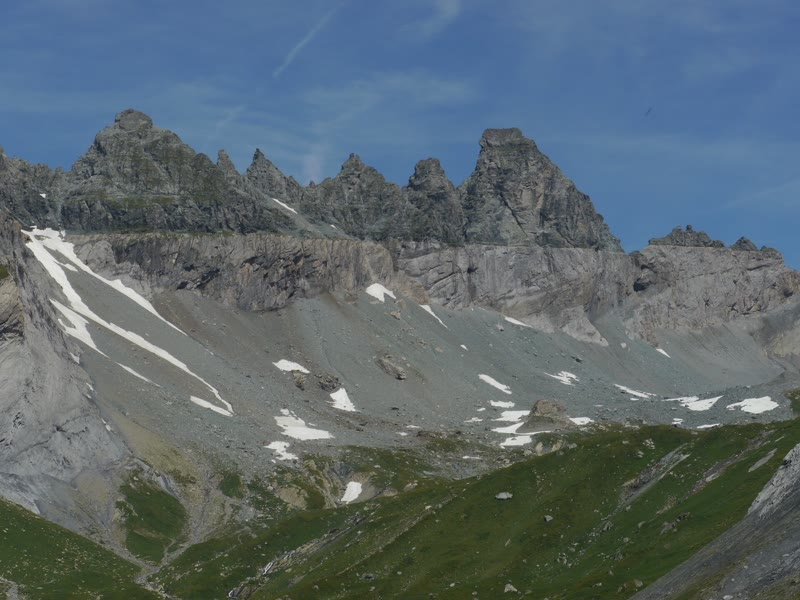
\includegraphics[width=0.5\linewidth]{images/book2/g12-heine-glarus-thrust.jpg}

{\small पूर्वी स्विट्ज़रलैंड के आल्प्स में ग्लारुस \omterm{def:g12:mountain-building:thrust}{प्रणोद}। चोटियों की गहरी
चट्टानें, जो पर्मियन में, लगभग 299 और 252
मिलियन वर्ष पहले के बीच, जमी थीं, हल्की और कहीं अधिक नई चट्टानों पर टिकी हैं; \omterm{def:g12:mountain-building:thrust}{प्रणोद}
उनके बीच की तीखी सीमा है। ऊपरी चट्टानें लगभग 40 से
\qty{50}{km} खिसकी हैं। फ़ोटो क्रिस्टियान हाइने (CC~BY-SA~3.0)।}
\end{omfigure}
% ledger: photo:g12-glarus (Verrucano, Permian; displacement 40-50 km, Pfiffner 1985), ics:base.Permian, ics:base.Triassic

\subsection{लघुकरण का मापन}

\omterm{def:g12:mountain-building:fold}{वलन} और \omterm{def:g12:mountain-building:thrust}{प्रणोद} दोनों भूपर्पटी को उस दिशा में छोटा करते हैं जिसमें वह
भींची जाती है।

\begin{definition}[लघुकरण]\label{def:g12:mountain-building:shortening}
किसी परत का \emph{लघुकरण}\index{लघुकरण} उसकी लंबाई का वह अंश है जो
उसने खो दिया है: यदि वह $L_0$ लंबी थी और अब $L$ तक फैली है,
\[
  e = \frac{L_0 - L}{L_0}.
\]
\end{definition}

इसे मापने के लिए मूल लंबाई $L_0$ चाहिए। बहुत-से \omterm{def:g12:mountain-building:fold}{वलनों} में
परतें मुड़ते हुए अपनी मोटाई बनाए रखती हैं, एक-दूसरे पर ऐसे सरकती हुई जैसे
मुड़ी किताब के पन्ने; ऐसी परत अपनी लंबाई के अनुदिश खिंचती नहीं। इससे
मूल लंबाई मिल जाती है।
% ledger: tulane:fold-geometry (flexural folds keep their thickness)

\begin{proposition}[मुड़ी परत का लघुकरण]\label{prop:g12:mountain-building:shortening}
यदि कोई परत अपने अनुदिश खिंचे या भिंचे बिना मुड़ी है, तो
उसकी मूल लंबाई $L_0$ मुड़ी परत के अनुदिश मापी गई उसकी लंबाई है।
कोण $\theta$ पर नत सीधी भुजाओं वाले \omterm{def:g12:mountain-building:fold}{वलन} के लिए,
\[
  e = 1 - \cos\theta .
\]
\end{proposition}

\begin{proof}
परत को बिना खींचे खोलने पर वह अपनी लंबाई बदले बिना समतल
बिछ जाती है; इसलिए $L_0$ परत के अनुदिश की लंबाई है। किसी सीधी भुजा पर,
जिसकी लंबाई $\ell$ है और जो $\theta$ पर नत है, तय की गई
क्षैतिज दूरी $\ell\cos\theta$ है (समकोण त्रिभुज)। सभी भुजाओं को जोड़ने पर
लंबाई $L_0$ की परत $L = L_0\cos\theta$ तक फैलती है, और $e = (L_0 - L_0\cos\theta)/L_0 =
1 - \cos\theta$।
\end{proof}

\begin{omfigure}
\begin{tikzpicture}
\begin{axis}[name=sine, x=2.0cm, y=2.0cm, axis lines=none,
  xmin=-0.05, xmax=2.25, ymin=-0.4, ymax=0.8, clip=false]
% computed in figdata/grade-12/fold_shortening.py (part sine: A/lambda = 0.25, e = 31.7 %)
\addplot[omLithSand!80!black, line width=1.6pt] table[x=x, y=y] {figdata/out/grade-12-fold_shortening-sine.dat};
\draw[omThm, line width=1.6pt] (axis cs:0,0.62) -- (axis cs:2.196,0.62);
\draw[black!60, |-|] (axis cs:0,-0.32) -- node[below, font=\scriptsize] {$L$ (आज)} (axis cs:1.5,-0.32);
\node[anchor=south west, font=\scriptsize, omThm] at (axis cs:0,0.64) {$L_0$: वही परत, खोली हुई};
\end{axis}
\begin{axis}[omrecord, at={(sine.east)}, anchor=west, xshift=1.4cm, width=0.46\linewidth, height=4.6cm,
  xmin=0, xmax=80, ymin=0, ymax=85, xlabel={भुजा का नमन $\theta$ (\unit{\degree})},
  ylabel={लघुकरण $e$ (\unit{\percent})}, xtick={0,20,...,80}]
% computed in figdata/grade-12/fold_shortening.py (part dip: e = 1 - cos theta)
\addplot[omProp, line width=1pt] table[x=theta, y=e_pct] {figdata/out/grade-12-fold_shortening-dip.dat};
\addplot[only marks, mark=*, mark size=1.6pt, omThm] coordinates {(12,2.185) (30,13.397) (60,50)};
\node[anchor=south, font=\scriptsize, align=center] at (axis cs:12,6) {वार्डन:\\\qty{2.2}{\percent}};
\node[anchor=west, font=\scriptsize] at (axis cs:32,10) {\qty{13}{\percent}};
\node[anchor=south east, font=\scriptsize] at (axis cs:60,51) {\qty{50}{\percent}};
\end{axis}
\end{tikzpicture}

{\small बाएँ: एक मुड़ी परत $L$ तक फैली है; बिना
खींचे समतल बिछाने पर वह $L_0$ लंबी है (यहाँ \omterm{def:g12:mountain-building:fold}{वलन} अपनी तरंगदैर्घ्य के एक-चौथाई जितने
ऊँचे हैं, और $L$, $L_0$ का \qty{68}{\percent} है)। दाएँ: सीधी भुजाओं वाले \omterm{def:g12:mountain-building:fold}{वलन} का
\omterm{def:g12:mountain-building:shortening}{लघुकरण}, $1 - \cos\theta$, उसकी भुजाओं के नमन के
सापेक्ष। मंद \omterm{def:g12:mountain-building:fold}{वलन} किसी परत को बहुत कम छोटा करते हैं।}
\end{omfigure}
% values: sine_025_e_pct 31.68 (L/L0 = 0.683); varden_e_pct 2.1852; chevron_30 13.397; chevron_60 50 (fold_shortening.py)

\begin{method}[काट पर लघुकरण का मापन]\label{met:g12:mountain-building:shortening}
\begin{enumerate}
  \item जाँचिए कि काट वास्तविक पैमाने पर खींची गई है। यदि उसका ऊर्ध्वाधर पैमाना
        खींचा गया है, तो नमन और परतों के अनुदिश लंबाइयाँ बहुत बड़ी होती हैं: उसे
        फिर से खींचिए, या पहले हर नमन सुधारिए।
  \item परत की एक ऐसी सीमा चुनिए जिसका काट के आर-पार अनुसरण किया जा सके;
        जहाँ कोई भ्रंश उसे काटता है, वहाँ दोनों कटे सिरों को वैसे जोड़िए जैसे वे भ्रंश
        खिसकने से पहले थे।
  \item परत के अनुदिश उसकी लंबाई, $L_0$, मापिए: किसी धागे से उसका अनुसरण कीजिए,
        या छोटे सीधे टुकड़ों को जोड़िए।
  \item उसके दोनों सिरों के बीच की क्षैतिज दूरी, $L$, मापिए।
  \item $e = (L_0 - L)/L_0$ परिकलित कीजिए; ज्ञात नमन की सीधी भुजाओं के लिए
        $e = 1 - \cos\theta$ इसे तुरंत देता है।
\end{enumerate}
\end{method}

\begin{example}[वार्डन के वलन]\label{ex:g12:mountain-building:varden}
वार्डन \omterm{def:g12:mountain-building:fold}{वलनों} की भुजाएँ \ang{12} नत हैं, इसलिए आवरण का \omterm{def:g12:mountain-building:shortening}{लघुकरण}
$e = 1 - \cos\ang{12} = 1 - 0.978 = 0.022$ हुआ, लगभग \qty{2.2}{\percent}: क्षेत्र की
जो पट्टी आज \qty{10}{km} चौड़ी है, वह \omterm{def:g12:mountain-building:fold}{वलन} से पहले $10/\cos\ang{12} \approx
\qty{10.22}{km}$ चौड़ी थी। काट A--B पर जैसी खींची गई है वैसी मापने पर
भुजाएँ लगभग \ang{28} खड़ी दिखतीं, क्योंकि ऊर्ध्वाधर पैमाना
2.5 गुना खींचा गया है: $\tan\theta$ 2.5 से गुणा हो जाता है, और $\arctan(2.5
\tan\ang{12}) \approx \ang{28}$। ज्यों का त्यों पढ़ने पर यह
\qty{12}{\percent} का \omterm{def:g12:mountain-building:shortening}{लघुकरण} देता, पाँच गुना से भी अधिक।
\end{example}
% values: varden_e_pct 2.1852, varden_L0_for_10km 10.223 (fold_shortening.py); arctan(2.5 x 0.2126) = 27.98 deg; 1 - cos 27.98 = 0.117

मंद \omterm{def:g12:mountain-building:fold}{वलन} कम अवशोषित करते हैं। कसकर मुड़ी पट्टी, जिसकी भुजाएँ
\ang{60} नत हों, आधी छोटी हो चुकी होती है; और कोई एक लगभग समतल \omterm{def:g12:mountain-building:thrust}{प्रणोद} जिसने
किसी \omterm{def:g12:mountain-building:nappe}{नैप} को \qty{40}{km} ढोया है, \qty{40}{km} \omterm{def:g12:mountain-building:shortening}{लघुकरण} अवशोषित करता है, उतना ही
जितना मंद \omterm{def:g12:mountain-building:fold}{वलनों} की एक बहुत चौड़ी पट्टी।

\section{मोटा होना और उत्थान}

\omterm{def:g12:mountain-building:shortening}{लघुकरण} चट्टान को नष्ट नहीं करता। भूपर्पटी की जो पट्टी अपनी पूर्व चौड़ाई के एक अंश तक
भींची गई है, वह अपना आयतन बनाए रखती है, इसलिए उसे मोटा होना ही पड़ता है: यदि
$H_0$ मोटी भूपर्पटी पट्टी की पूरी लंबाई के अनुदिश चौड़ाई $L_0$ से $L$ तक छोटी की जाए,
तो उसकी अनुप्रस्थ काट अपना क्षेत्रफल बनाए रखती है, $H L = H_0 L_0$, और
\[
  H = H_0\,\frac{L_0}{L} = \frac{H_0}{1 - e}.
\]
\qty{50}{\percent} छोटी की गई \qty{35}{km} मोटी भूपर्पटी
\qty{70}{km} मोटी हो जाती है। फिर \omterm{def:g11:lithosphere-asthenosphere:isostasy}{समस्थिति} बाक़ी काम करती है: अधिक मोटी भूपर्पटी अधिक
ऊँची तैरती है, अधिक गहरे \omterm{def:g12:continental-crust:root}{मूल} के ऊपर (\cref{prop:g11:lithosphere-asthenosphere:airy})।
एयरी के मॉडल और स्मरण के घनत्वों के साथ, जो भूपर्पटी
$\Delta H$ अधिक मोटी है वह $\Delta H\,(\rho_m - \rho_c)/\rho_m = \Delta H
\times 550/3380$ अधिक ऊँची खड़ी होती है, अतिरिक्त मोटाई का लगभग छठा भाग; बाक़ी पाँच
छठे भाग \omterm{def:g12:continental-crust:root}{मूल} बनाते हैं। पर्वत-पट्टियों से दूर भूपर्पटी \num{35} से \qty{40}{km} मोटी है,
और उनके नीचे 50 से \qty{70}{km}: पर्वत जितने ऊँचे,
भूपर्पटी उतनी मोटी।
% ledger: tulane:roots, cm95:crust, data:prem

इसी तरह समुद्री तली का चूना पत्थर एवरेस्ट की चोटी पर पहुँचा: किसी समुद्र की
तली पर जमकर, वह भारत के साथ उत्तर की ओर ले जाया गया, हिमालय की प्रणोद-चादरों में
तहों में चढ़ाया गया, और उसके नीचे की भूपर्पटी के मोटा होकर ऊपर उठने के साथ ऊपर उठा।
भूपर्पटी की ऐसी ऊर्ध्वाधर गति को उत्थान कहते हैं।
% ledger: sakai05:summit, sakai05:stacking, tulane:roots (uplift), usgs:himalaya-collision

\section{दो श्रेणियाँ}

\subsection{हिमालय}

हिमालय भारत और
तिब्बत की सीमा के अनुदिश \qty{2900}{km} तक फैला है। लगभग 80 मिलियन वर्ष पहले भारत
एशिया से लगभग \qty{6400}{km} दक्षिण में, एक महासागर के पार, था, और प्रति वर्ष लगभग
\qty{9}{cm} की दर से उत्तर की ओर चलता था; वह 40 और 50 मिलियन वर्ष पहले के बीच
एशिया से मिला, और तब उसका उत्तर की ओर बढ़ना
धीमा हो गया। प्लेट-पुनर्निर्माण इस यात्रा को विस्तार से दिखाते हैं: बहुत-से
प्रकार के प्रमाणों से बने, जिनमें तप्त स्थलों के पथ भी हैं
(\cref{ch:g11:plate-motions}), वे प्लेटों को समय में पीछे क़दम-दर-क़दम
ले जाते हैं।
% ledger: usgs:himalaya-collision, muller19:frame, muller22:frame

\begin{omfigure}
\begin{tikzpicture}
\begin{axis}[omrecord, omage, name=lat, width=0.5\linewidth, height=5.2cm,
  xmin=0, xmax=100, ymin=-45, ymax=35, xlabel={आयु (\unit{Ma})}, ylabel={अक्षांश (\unit{\degree})},
  xtick={0,20,...,100}, ytick={-40,-20,...,40},
  legend style={font=\scriptsize, at={(0.98,0.03)}, anchor=south east, fill=white}]
% computed in figdata/grade-12/india_drift.py (part lat; GPlates Web Service, MULLER2022 and MULLER2019)
\fill[omThm!12] (axis cs:40,-45) rectangle (axis cs:50,35);
\addplot[omThm, line width=1.1pt] table[x=age, y=m22_india] {figdata/out/grade-12-india_drift-lat.dat};
\addplot[omThm, dashed, line width=0.8pt] table[x=age, y=m19_india] {figdata/out/grade-12-india_drift-lat.dat};
\addplot[omDef, line width=1.1pt] table[x=age, y=m22_lhasa] {figdata/out/grade-12-india_drift-lat.dat};
\addplot[black!50, line width=0.4pt, forget plot] coordinates {(0,0) (100,0)};
\legend{{मध्य भारत (2022)}, {मध्य भारत (2019)}, {ल्हासा (2022)}}
\end{axis}
\begin{axis}[omrecord, omage, at={(lat.east)}, anchor=west, xshift=1.9cm, width=0.42\linewidth, height=5.2cm,
  xmin=0, xmax=100, ymin=0, ymax=160, xlabel={आयु (\unit{Ma})},
  ylabel={उत्तर की ओर चाल (\unit{mm/yr})}, xtick={0,20,...,100}]
% computed in figdata/grade-12/india_drift.py (part steps: 5-Myr steps)
\fill[omThm!12] (axis cs:40,0) rectangle (axis cs:50,160);
\addplot[omThm, line width=1pt] table[x=age, y=m22] {figdata/out/grade-12-india_drift-steps.dat};
\addplot[omThm, dashed, line width=0.7pt] table[x=age, y=m19] {figdata/out/grade-12-india_drift-steps.dat};
\end{axis}
\end{tikzpicture}

{\small बाएँ: मध्य भारत के एक बिंदु (आज \ang{78}~पू,
\ang{20}~उ) और \omterm{def:g12:mountain-building:suture}{सीवन} के उत्तर में ल्हासा का अक्षांश, पिछले 100
मिलियन वर्षों में, दो प्रकाशित प्लेट-पुनर्निर्माणों (2022 और 2019) में।
दाएँ: 5 मिलियन वर्ष के हर चरण में भारत की उत्तर की ओर चाल। छायांकित
पट्टी 40 से 50 मिलियन वर्ष पहले को चिह्नित करती है। आँकड़े: आर॰~डी॰~म्यूलर और सहयोगी
(2019, 2022), जीप्लेट्स वेब सेवा से परिकलित।}
\end{omfigure}
% ledger: data:b2-gws-india, muller22:frame, muller19:frame; values: speed_65_50 128.5, speed_40_0 40.06, fastest 145.8 (50-55 Ma) (india_drift.py)

दोनों पुनर्निर्माण कुछ अंशों के भीतर सहमत हैं। 65 और 50 मिलियन
वर्ष पहले के बीच भारत प्रति वर्ष लगभग \qty{13}{cm} उत्तर की ओर चला; 50 और 40
मिलियन वर्ष पहले के बीच उसकी चाल गिरी, और
40 मिलियन वर्ष पहले से वह प्रति वर्ष लगभग \qty{4}{cm} चला है, एक-तिहाई
से भी कम। एशियाई ओर का ल्हासा भी उत्तर की ओर चला, पर कहीं
अधिक धीरे।
% values: speed_65_50 128.5 mm/yr, speed_40_0 40.06 mm/yr, slowdown_ratio 0.312 (india_drift.py)

\begin{example}[भारत की चाल]\label{ex:g12:mountain-building:india}
2022 के पुनर्निर्माण में मध्य भारत 60 मिलियन
वर्ष पहले \ang{12.10}~द पर और 50 मिलियन वर्ष पहले \ang{0.68}~द पर था। अक्षांश का एक अंश
$2\pi R/360 = 2\pi \times \qty{6371}{km}/360 \approx \qty{111.2}{km}$ है। भारत
10 मिलियन वर्षों में $(12.10 - 0.68) \times 111.2 \approx \qty{1270}{km}$ उत्तर की ओर चला:
प्रति मिलियन वर्ष \qty{127}{km}, यानी $\qty{127e6}{mm} /
\num{e6}\text{ वर्ष} = \qty{127}{mm}$, लगभग \qty{13}{cm}, प्रति वर्ष।
\end{example}
% ledger: data:b2-gws-india, earth:Rmean; values: lat 60 Ma -12.0964, 50 Ma -0.6801 (india_drift-lat)

इस धीमेपन को टक्कर का चिह्न माना जाता है: खाई तक पहुँचती
\omterm{def:g12:continental-crust:continental-crust}{महाद्वीपीय भूपर्पटी} डूब नहीं सकी, और भारत रोक लिया गया। पहले संपर्क की सटीक तिथि पर अब भी बहस है: अनुमान
लगभग 60 से 54 मिलियन वर्ष पहले तक हैं, और कुछ भूवैज्ञानिकों का तर्क है कि
भारत पहले ज्वालामुखीय द्वीपों की एक श्रृंखला से मिला और स्वयं एशिया तक केवल
लगभग 34 मिलियन वर्ष पहले पहुँचा। भारत रुका नहीं है: आज की प्लेटों के घूर्णन ध्रुव
उसे हिमालय के आर-पार प्रति वर्ष लगभग \qty{4.5}{cm} की दर से यूरेशिया की ओर ले जाते हैं
(\cref{ch:g11:plate-motions}), और यह दबाव एशिया के कुछ भागों को
पूर्व की ओर भींचता है।
% ledger: usgs:himalaya-collision, najman21:collision-age; values: today_in_eu_speed 44.99 mm/yr (india_drift.py, from nnr56:poles)

हिमालय के उत्तर में तिब्बत का पठार औसतन लगभग \qty{4600}{m} ऊँचा खड़ा है,
लगभग \qty{70}{km} मोटी भूपर्पटी के ऊपर
(\cref{ch:g11:lithosphere-asthenosphere})। भारत और तिब्बत के बीच
अपने \omterm{def:g12:mountain-building:ophiolite}{ओफ़ियोलाइटों} के साथ सिंधु--त्सांगपो \omterm{def:g12:mountain-building:suture}{सीवन} है; उसके दक्षिण में हिमालय
ज़्यादातर भारत के उत्तरी किनारे पर जमे अवसादों से बना है, जो फिर तहों में चढ़े,
मुड़े और भ्रंशित हुए, उनमें एवरेस्ट की चोटी का चूना पत्थर भी।
% ledger: karplus:tibet-moho, liu20:itsz, sakai05:stacking, sakai05:summit; Book 1: usgs:himalaya (Tibetan Plateau about 4600 m)

\subsection{आल्प्स, और एक पूरी पट्टी}

आल्प्स का इतिहास छोटे पैमाने पर मिलता-जुलता है: वे वहाँ उठे जहाँ अफ़्रीका
यूरोप से टकराया। उनमें भी \omterm{def:g12:mountain-building:ophiolite}{ओफ़ियोलाइट} हैं, और बड़े \omterm{def:g12:mountain-building:thrust}{प्रणोद}: ग्लारुस
प्रणोद पर पर्मियन चट्टानें कहीं अधिक नई चट्टानों के ऊपर ले जाई गई हैं।
आल्प्स और हिमालय पर्वतों की एक लंबी पट्टी के अंग हैं, जो ईरान के
ज़ाग्रोस से होकर जाती है, जहाँ अफ़्रीका और भारत यूरेशिया से टकराए हैं।
% ledger: earle:collision, photo:g12-glarus

\begin{omfigure}
\begin{tikzpicture}
\begin{axis}[axis equal image, xmin=-12, xmax=105, ymin=18, ymax=52, width=\linewidth,
  tick label style={font=\scriptsize}, xtick={0,30,60,90}, ytick={20,30,40,50},
  xticklabel={$\pgfmathprintnumber{\tick}^\circ$}, yticklabel={$\pgfmathprintnumber{\tick}^\circ$},
  axis background/.style={fill=omSea}, legend columns=3,
  legend style={font=\scriptsize, at={(0.5,-0.12)}, anchor=north, /tikz/every even column/.append style={column sep=5pt}}]
\addplot[fill=omLithAlluv, draw=black!45, line width=0.2pt, forget plot] table {figdata/out/shared-geo-land.dat};
% computed in figdata/grade-12/alpine_belt.py; ledger: data:etopo1, data:usgs-comcat
\addplot[only marks, mark=square*, mark size=1.15pt, omLithSand!85!black] table[x=lon, y=lat] {figdata/out/grade-12-alpine_belt-high.dat};
\addplot[only marks, mark=square*, mark size=1.15pt, omThm!75!black] table[x=lon, y=lat] {figdata/out/grade-12-alpine_belt-higher.dat};
\addplot[only marks, mark=*, mark size=0.7pt, black] table[x=lon, y=lat] {figdata/out/grade-12-alpine_belt-quakes.dat};
\addplot[omDef, line width=0.9pt, forget plot] table {figdata/out/shared-geo-school-collision.dat};
\addplot[black!70, line width=0.5pt, forget plot] table {figdata/out/shared-geo-school-subduction.dat};
\legend{{\qty{1500}{m} से ऊँचा}, {\qty{3500}{m} से ऊँचा}, {भूकंप, परिमाण 6 या अधिक}}
\coordinate (alps) at (axis cs:9,48);
\coordinate (zagros) at (axis cs:46,23.5);
\coordinate (zagrosbelt) at (axis cs:50.5,31.5);
\coordinate (himal) at (axis cs:84,24);
\coordinate (tibet) at (axis cs:88,33);
\coordinate (arrA) at (axis cs:77,19.5);
\coordinate (arrB) at (axis cs:79.2,25);
\end{axis}
% labels drawn after the axis, so that no earthquake dot covers them
\node[font=\scriptsize, fill=white, inner sep=1pt, anchor=south] at (alps) {आल्प्स};
\draw[black!60, line width=0.4pt] (zagros) -- (zagrosbelt);
\node[font=\scriptsize, fill=white, inner sep=1pt] at (zagros) {ज़ाग्रोस};
\node[font=\scriptsize, fill=white, inner sep=1pt, anchor=west] at (himal) {हिमालय};
\node[font=\scriptsize, fill=white, inner sep=1pt] at (tibet) {तिब्बत का पठार};
\draw[-{Stealth[length=2mm]}, line width=1pt, omProp] (arrA) -- (arrB);
\end{tikzpicture}

{\small अटलांटिक से तिब्बत तक नए पर्वतों की पट्टी: ऊँची भूमि
(हर वर्ग 1-अंश की एक कोशिका है), 1976 से 2025 तक परिमाण 6 या अधिक के उथले भूकंप
(\qty{70}{km} से उथले), और प्लेटों के बीच की टक्कर-सीमाएँ
(नीली रेखा)। तीर यूरेशिया की ओर भारत की गति दिखाता है।
आँकड़े: ETOPO1, USGS भूकंप-सूची, बर्ड (2003) की प्लेट-सीमाएँ,
स्थल नैचुरल अर्थ से।}
\end{omfigure}
% ledger: data:etopo1, data:usgs-comcat, data:pb2002, data:ne-land; values: n_quakes 398 (alpine_belt.py)

ऊँची भूमि और भूकंप एक ही संकरी पट्टी का अनुसरण करते हैं।
टक्कर समाप्त नहीं हुई है: भूकंप दिखाते हैं कि पूरी पट्टी के अनुदिश भूपर्पटी अब भी टूट
रही है, और पर्वत अब भी बन रहे हैं।

\section{अभ्यास}

\begin{exercise}[$\star$]\label{exo:g12:mountain-building:1}
हर पद को उसके वर्णन से मिलाइए: \omterm{def:g12:mountain-building:fold}{अपनति}, \omterm{def:g12:mountain-building:fold}{अभिनति}, \omterm{def:g12:mountain-building:thrust}{प्रणोद}, \omterm{def:g12:mountain-building:nappe}{नैप},
\omterm{def:g12:mountain-building:suture}{सीवन}, \omterm{def:g12:mountain-building:ophiolite}{ओफ़ियोलाइट}। (a) मंद नमन वाला \omterm{def:g12:mountain-building:thrust}{उत्क्रम भ्रंश}; (b) स्थल पर मिला
महासागरीय तली का एक टुकड़ा; (c) वह \omterm{def:g12:mountain-building:fold}{वलन} जिसकी भुजाएँ उसके अक्ष की ओर नत हों;
(d) वह रेखा जहाँ दो महाद्वीप जुड़े थे; (e) वह \omterm{def:g12:mountain-building:fold}{वलन} जिसकी भुजाएँ
उसके अक्ष से दूर नत हों; (f) \omterm{def:g12:mountain-building:thrust}{प्रणोद} के अनुदिश दूर तक ले जाई गई चट्टान की एक बड़ी चादर।
\end{exercise}

\begin{exercise}[$\star$]\label{exo:g12:mountain-building:2}
एक घाटी के आर-पार, पश्चिमी ओर की परतें पश्चिम की ओर \ang{20} नत हैं और
पूर्वी ओर की परतें पूर्व की ओर \ang{20}। (1) उनके बीच का \omterm{def:g12:mountain-building:fold}{वलन}
\omterm{def:g12:mountain-building:fold}{अपनति} है या \omterm{def:g12:mountain-building:fold}{अभिनति}? (2) अपरदन के बाद उसके अक्ष के अनुदिश सबसे पुरानी परतें मिलती हैं या सबसे नई?
(3) क्या घाटी का किसी \omterm{def:g12:mountain-building:fold}{अभिनति} के ऊपर होना आवश्यक है?
\end{exercise}

\begin{exercise}[$\star$]\label{exo:g12:mountain-building:3}
एक परत \ang{30} पर नत सीधी भुजाओं के साथ मुड़ी है। (1) उसका
\omterm{def:g12:mountain-building:shortening}{लघुकरण} परिकलित कीजिए। (2) आज वह \qty{6.0}{km} तक फैली है। वह कितनी लंबी थी?
\end{exercise}

\begin{exercise}[$\star$]\label{exo:g12:mountain-building:4}
(1) किसी भ्रंश के अनुदिश भ्रंश-तल के ऊपर का खंड नीचे खिसका है। यह
\omterm{def:g11:ocean-ridges:normal-fault}{सामान्य भ्रंश} है या उत्क्रम, और भूपर्पटी खिंची थी या भींची गई थी?
(2) एक \omterm{def:g12:mountain-building:thrust}{उत्क्रम भ्रंश} \ang{25} नत है: क्या यह \omterm{def:g12:mountain-building:thrust}{प्रणोद} है?
\end{exercise}

\begin{exercise}[$\star$]\label{exo:g12:mountain-building:5}
(1) किसी \omterm{def:g12:mountain-building:ophiolite}{ओफ़ियोलाइट} की इन चट्टानों को ऊपर से नीचे के क्रम में रखिए: \omterm{def:g11:ocean-ridges:gabbro}{गैब्रो},
समुद्री अवसाद, \omterm{def:g11:ocean-ridges:peridotite}{पेरिडोटाइट}, तकिया बेसाल्ट, चादरी \omterm{def:g11:igneous-rocks:intrusion}{डाइक}। (2) तकिया बेसाल्ट
क्यों दिखाते हैं कि चट्टान पानी के नीचे बनी? (3) \omterm{def:g12:mountain-building:ophiolite}{ओफ़ियोलाइट}
\omterm{def:g12:mountain-building:suture}{सीवनों} के अनुदिश क्यों मिलते हैं?
\end{exercise}

\begin{exercise}[$\star\star$]\label{exo:g12:mountain-building:6}
वास्तविक पैमाने की एक काट पर, बलुआ पत्थर की एक सीमा का चार
सीधे टुकड़ों के आर-पार अनुसरण किया जाता है, जो \qty{2.1}{km}, \qty{1.8}{km}, \qty{2.4}{km} और
\qty{1.6}{km} लंबे हैं; उसके सिरे \qty{6.0}{km} दूर हैं। (1)
\omterm{def:g12:mountain-building:shortening}{लघुकरण} परिकलित कीजिए। (2) यदि चारों भुजाएँ एक ही कोण पर नत हों, तो वह कोण क्या है?
\end{exercise}

\begin{exercise}[$\star\star$]\label{exo:g12:mountain-building:7}
\ang{10} नत किसी \omterm{def:g12:mountain-building:thrust}{प्रणोद} का ऊपरी खंड भ्रंश-तल के अनुदिश \qty{45}{km}
खिसका है। (1) वह क्षैतिज रूप से कितना खिसका है? (2) वह कितना
ऊपर उठा है? (3) \ang{12} नत भुजाओं वाले \omterm{def:g12:mountain-building:fold}{वलनों} की कितनी चौड़ी पट्टी
उतना ही क्षैतिज \omterm{def:g12:mountain-building:shortening}{लघुकरण} अवशोषित करेगी?
\end{exercise}

\begin{exercise}[$\star\star$]\label{exo:g12:mountain-building:8}
मैककॉनेल प्रणोद के अनुदिश लगभग 500 मिलियन वर्ष पुराना चूना पत्थर
लगभग 75 मिलियन वर्ष पुराने पंकाश्म पर पड़ा है। (1) सापेक्ष काल-निर्धारण का कौन-सा सिद्धांत
भ्रंश की उपेक्षा करने वाले भूवैज्ञानिक को भ्रमित करेगा? (2) ऊपरी चट्टान कितनी
अधिक पुरानी है? (3) प्रणोद-चादर लगभग \qty{800}{m} मोटी है और
\qty{40}{km} खिसकी है: यह उसकी अपनी मोटाई का कितना गुना है?
\end{exercise}

\begin{exercise}[$\star\star$]\label{exo:g12:mountain-building:9}
2022 के पुनर्निर्माण में मध्य भारत 80 मिलियन
वर्ष पहले \ang{30.23}~द पर और 66 मिलियन वर्ष पहले \ang{19.38}~द पर था। (1) वह उत्तर की ओर कितना
चला? (2) किस माध्य चाल से, \unit{cm} प्रति वर्ष में? (3) अमेरिकी भूवैज्ञानिक सर्वेक्षण के
सारांश, लगभग प्रति शताब्दी \qty{9}{m}, से तुलना कीजिए।
\end{exercise}

\begin{exercise}[$\star\star$]\label{exo:g12:mountain-building:10}
\qty{35}{km} मोटी भूपर्पटी पूरी पट्टी के आर-पार \qty{40}{\percent}
छोटी की जाती है। (1) वह कितनी मोटी हो जाती है? (2) $\rho_c =
\qty{2830}{kg/m^3}$ और $\rho_m = \qty{3380}{kg/m^3}$ के साथ वह कितनी ऊँची
खड़ी होती है, और उसका अतिरिक्त \omterm{def:g12:continental-crust:root}{मूल} कितना गहरा है?
\end{exercise}

\begin{exercise}[$\star\star$]\label{exo:g12:mountain-building:11}
3 गुना खींचे ऊर्ध्वाधर पैमाने वाली काट पर कोई भुजा \ang{40} नत
दिखती है। (1) उसका वास्तविक नमन क्या है? (2) वास्तविक
नमन से और चित्र पर पढ़े नमन से \omterm{def:g12:mountain-building:shortening}{लघुकरण} परिकलित कीजिए। (3) \omterm{def:g12:mountain-building:shortening}{लघुकरण} मापने के लिए
उपयोग की जाने वाली काटें वास्तविक पैमाने पर क्यों खींची जानी चाहिए?
\end{exercise}

\begin{exercise}[$\star\star\star$]\label{exo:g12:mountain-building:12}
इस अध्याय में खींचे गए गोल \omterm{def:g12:mountain-building:fold}{वलन}, जो अपनी तरंगदैर्घ्य के एक-चौथाई जितने
ऊँचे हैं, का \omterm{def:g12:mountain-building:shortening}{लघुकरण} \qty{31.7}{\percent} है; उनका सबसे तीव्र नमन
लगभग \ang{57.5} है। (1) इस तरह मुड़ी परत \qty{10}{km} तक फैली है: वह कितनी लंबी
थी? (2) \ang{57.5} पर सीधी भुजाओं वाले \omterm{def:g12:mountain-building:fold}{वलन} का \omterm{def:g12:mountain-building:shortening}{लघुकरण} परिकलित
कीजिए। (3) समझाइए कि उसी सबसे तीव्र नमन के लिए सीधी भुजाओं वाला \omterm{def:g12:mountain-building:fold}{वलन}
अधिक छोटा क्यों करता है।
\end{exercise}

\begin{exercise}[$\star\star\star$]\label{exo:g12:mountain-building:13}
हिमालय के उत्तर में, \ang{85}~पू \ang{28}~उ पर, घूर्णन ध्रुव भारत को
यूरेशिया के सापेक्ष \qty{16.6}{mm/yr} पूर्व की ओर और
\qty{41.8}{mm/yr} उत्तर की ओर का वेग देते हैं। पिछले 5 मिलियन वर्षों में 2022 का
पुनर्निर्माण मध्य भारत को ल्हासा की अपेक्षा \qty{23.5}{mm/yr}
अधिक उत्तर की ओर की चाल देता है। (1) यूरेशिया के सापेक्ष भारत की चाल
ज्ञात कीजिए। (2) यह मानकर कि उत्तर-घटकों की तुलना की जा सकती है, बताइए कि
ल्हासा के उत्तर के क्षेत्र के लिए प्रति मिलियन वर्ष कितना उत्तर--दक्षिण
\omterm{def:g12:mountain-building:shortening}{लघुकरण} बचता है? (3) अध्याय में कहाँ संकेत है कि यह क्षेत्र विकृत हो रहा है?
\end{exercise}

\begin{exercise}[$\star\star\star$]\label{exo:g12:mountain-building:14}
आल्प्स में एक \omterm{def:g12:mountain-building:nappe}{नैप} ऐसे \omterm{def:g12:mountain-building:thrust}{प्रणोद} के अनुदिश \qty{45}{km} ले जाया गया है जिसका नमन
लगभग शून्य है। (1) उस \omterm{def:g12:mountain-building:thrust}{प्रणोद} ने कितना \omterm{def:g12:mountain-building:shortening}{लघुकरण} अवशोषित किया? (2) वार्डन पहाड़ियों
जैसे मुड़े आवरण (भुजाएँ \ang{12}) की, \omterm{def:g12:mountain-building:fold}{वलन} से पहले की, कितनी चौड़ाई
उतना ही \omterm{def:g12:mountain-building:shortening}{लघुकरण} अवशोषित करेगी? (3) इससे क्या पता चलता है कि
पर्वत-पट्टियाँ बड़े अभिसरण कैसे अवशोषित करती हैं?
\end{exercise}

\begin{exercise}[$\star\star\star$]\label{exo:g12:mountain-building:15}
एवरेस्ट की चोटी का चूना पत्थर किसी समुद्री तली पर, समुद्र-तल से कम से कम
थोड़ा नीचे, जमा था, और आज \qty{8848.86}{m} पर खड़ा है। (1) यह मानकर कि
टक्कर 50 मिलियन वर्ष पहले शुरू हुई, उत्थान की न्यूनतम माध्य
दर, \unit{mm} प्रति वर्ष में, क्या है? (2) इसकी तुलना 40 मिलियन वर्ष पहले से भारत की
चाल, प्रति वर्ष लगभग \qty{40}{mm}, से कीजिए। (3) चट्टान का उत्थान
संभवतः उसकी वर्तमान ऊँचाई से अधिक क्यों है?
\end{exercise}

\begin{problem}[{सप्ताहांत समस्या --- भारत की यात्रा}]
\label{pb:g12:mountain-building:1}
% ledger: data:b2-gws-india, earth:Rmean, usgs:himalaya-collision, tulane:roots, cm95:crust, data:prem, karplus:tibet-moho; Book 1: usgs:himalaya (4600 m)
% values: india_drift-lat (MULLER2022, rounded to 0.01 deg); north_since_66_km 4378.7; converge_since_50 1354; gap_0 1073
तालिका 2022 के प्लेट-पुनर्निर्माण में मध्य भारत के एक बिंदु और \omterm{def:g12:mountain-building:suture}{सीवन} के उत्तर में
ल्हासा का अक्षांश देती है (ऋणात्मक = दक्षिण)।
अक्षांश का एक अंश \qty{111.2}{km} मानिए, और प्रति मिलियन
वर्ष \qty{1}{km} को प्रति वर्ष \qty{1}{mm}।

\begin{center}
\small
\begin{tabular}{|l|c|c|c|c|c|c|c|c|c|}
\hline
आयु (\unit{Ma}) & 80 & 66 & 60 & 55 & 50 & 45 & 40 & 20 & 0 \\ \hline
भारत (\unit{\degree}) & $-30.23$ & $-19.38$ & $-12.10$ & $-7.24$ & $-0.68$ & 3.30 & 5.59 & 13.40 & 20.00 \\ \hline
ल्हासा (\unit{\degree}) & & 19.48 & & & 21.15 & & & & 29.65 \\ \hline
\end{tabular}
\end{center}

\medskip
\noindent\textbf{भाग I --- अक्षांश और चालें।}
\begin{enumerate}
  \item $R =
        \qty{6371}{km}$ के साथ एक अंश के लिए \qty{111.2}{km} का मान जाँचिए।
  \item मध्य भारत ने भूमध्य रेखा कब पार की?
  \item 66 से 50 मिलियन वर्ष पहले तक भारत उत्तर की ओर कितना चला?
  \item किस माध्य चाल से?
  \item 66 से 40 मिलियन वर्ष पहले तक के हर चरण में उसकी चाल परिकलित कीजिए (66
        से 60, 60 से 55, इत्यादि)। वह किस चरण में सबसे तेज़ था?
\end{enumerate}

\medskip
\noindent\textbf{भाग II --- धीमापन।}
\begin{enumerate}[resume]
  \item 40 मिलियन वर्ष पहले से आज तक भारत की माध्य चाल परिकलित कीजिए।
  \item यह 66 से 50 मिलियन वर्ष पहले तक की उसकी चाल का कितना अंश है?
  \item तालिका की किन दो तिथियों के बीच चाल सबसे अधिक गिरी?
  \item टक्कर प्लेट को धीमा क्यों करती है?
  \item 50 मिलियन वर्ष पहले से आज तक भारत उत्तर की ओर कितना चला?
\end{enumerate}

\medskip
\noindent\textbf{भाग III --- अवशोषित अभिसरण।}
\begin{enumerate}[resume]
  \item 50 मिलियन वर्ष पहले से आज तक ल्हासा उत्तर की ओर कितना चला?
  \item 50 मिलियन वर्ष पहले से मध्य भारत और ल्हासा के बीच की
        उत्तर--दक्षिण दूरी कितनी घटी है?
  \item आज यह दूरी कितनी है, और 50 मिलियन वर्ष पहले कितनी थी?
  \item मान लीजिए यह सारा अभिसरण दोनों बिंदुओं के बीच की भूपर्पटी के
        \omterm{def:g12:mountain-building:shortening}{लघुकरण} से अवशोषित हुआ। \omterm{def:g12:mountain-building:shortening}{लघुकरण} $e$ क्या है?
  \item ऐसे \omterm{def:g12:mountain-building:shortening}{लघुकरण} को अवशोषित करने वाली दो प्रकार की संरचनाओं के नाम बताइए।
\end{enumerate}

\medskip
\noindent\textbf{भाग IV --- मोटी हुई भूपर्पटी।}
\begin{enumerate}[resume]
  \item यदि वह भूपर्पटी 50 मिलियन वर्ष पहले \qty{35}{km} मोटी थी, तो अपनी
        अनुप्रस्थ काट बनाए रखते हुए वह अब कितनी मोटी होगी?
  \item $\rho_c = \qty{2830}{kg/m^3}$ और $\rho_m = \qty{3380}{kg/m^3}$ के साथ
        वह अपने पूर्व स्तर से कितनी ऊँची खड़ी होगी?
  \item तिब्बत का पठार लगभग \qty{4600}{m} ऊँचा खड़ा है, लगभग
        \qty{70}{km} मोटी भूपर्पटी के ऊपर। एयरी का मॉडल \qty{4600}{m} के लिए
        भूपर्पटी की कौन-सी मोटाई देता है?
  \item एक कारण बताइए कि प्रश्न 16 का सरल मॉडल मोटा होने को
        अधिक क्यों आँकता है।
  \item प्रश्न 3 और 10 की दूरियाँ जोड़कर बताइए कि क्रिटेशस के अंत, 66 मिलियन वर्ष
        पहले, से भारत उत्तर की ओर कितनी
        यात्रा कर चुका है?
\end{enumerate}
\end{problem}
